%------------------------------------------------------------------------------
%	CRITERI DI TRASCRIZIONE
%------------------------------------------------------------------------------
\thispagestyle{empty}
\chapter*{Criteri di trascrizione}
La buona calligrafia di Mingazzi ha permesso una facile trascrizione e una discreta comprensione dei concetti che voleva comunicare.\:Tuttavia il testo contiene alcuni errori grammaticali e frasi poco chiare che non permettono la comprensione dell'elemento comico presente in ogni capitolo. Ho scelto quindi di riportare un consistente numero di note a piè di pagina per permettere la comprensione del testo e per arricchire la lettura con curiosità riguardanti i personaggi e i luoghi presentati. Consiglio fortemente di utilizzare queste note per meglio comprendere il testo e per apprendere alcune curiosità sui personaggi e i luoghi presentati. Il testo è stato riportato fedelmente dai manoscritti, ma ho apportato alcune modifiche al fine di una lettura più scorrevole. Per quanto riguarda i titoli dei capitoli ho voluto mantenere quelli dell'indice che si trova all'inizio dei sei quaderni. Siccome in alcuni capitoli vi sono dei sottocapitoli, ho separato questi da titoletti che non erano presenti nel testo originale. L'intero elaborato è stato scritto in \LaTeX\footnote{Scritto anche \LaTeX \: e pronunciato /ˈlatek/ in italiano; errato /ˈlateks/), è un linguaggio di markup usato per la preparazione di testi basato sul programma di composizione tipografica \TeX.} \:dal sottoscritto.\newpage
\noindent Di seguito una foto dell'indice originale:\\
 \begin{figure}[htb]
    \centering
    \vspace{-0.7cm}
    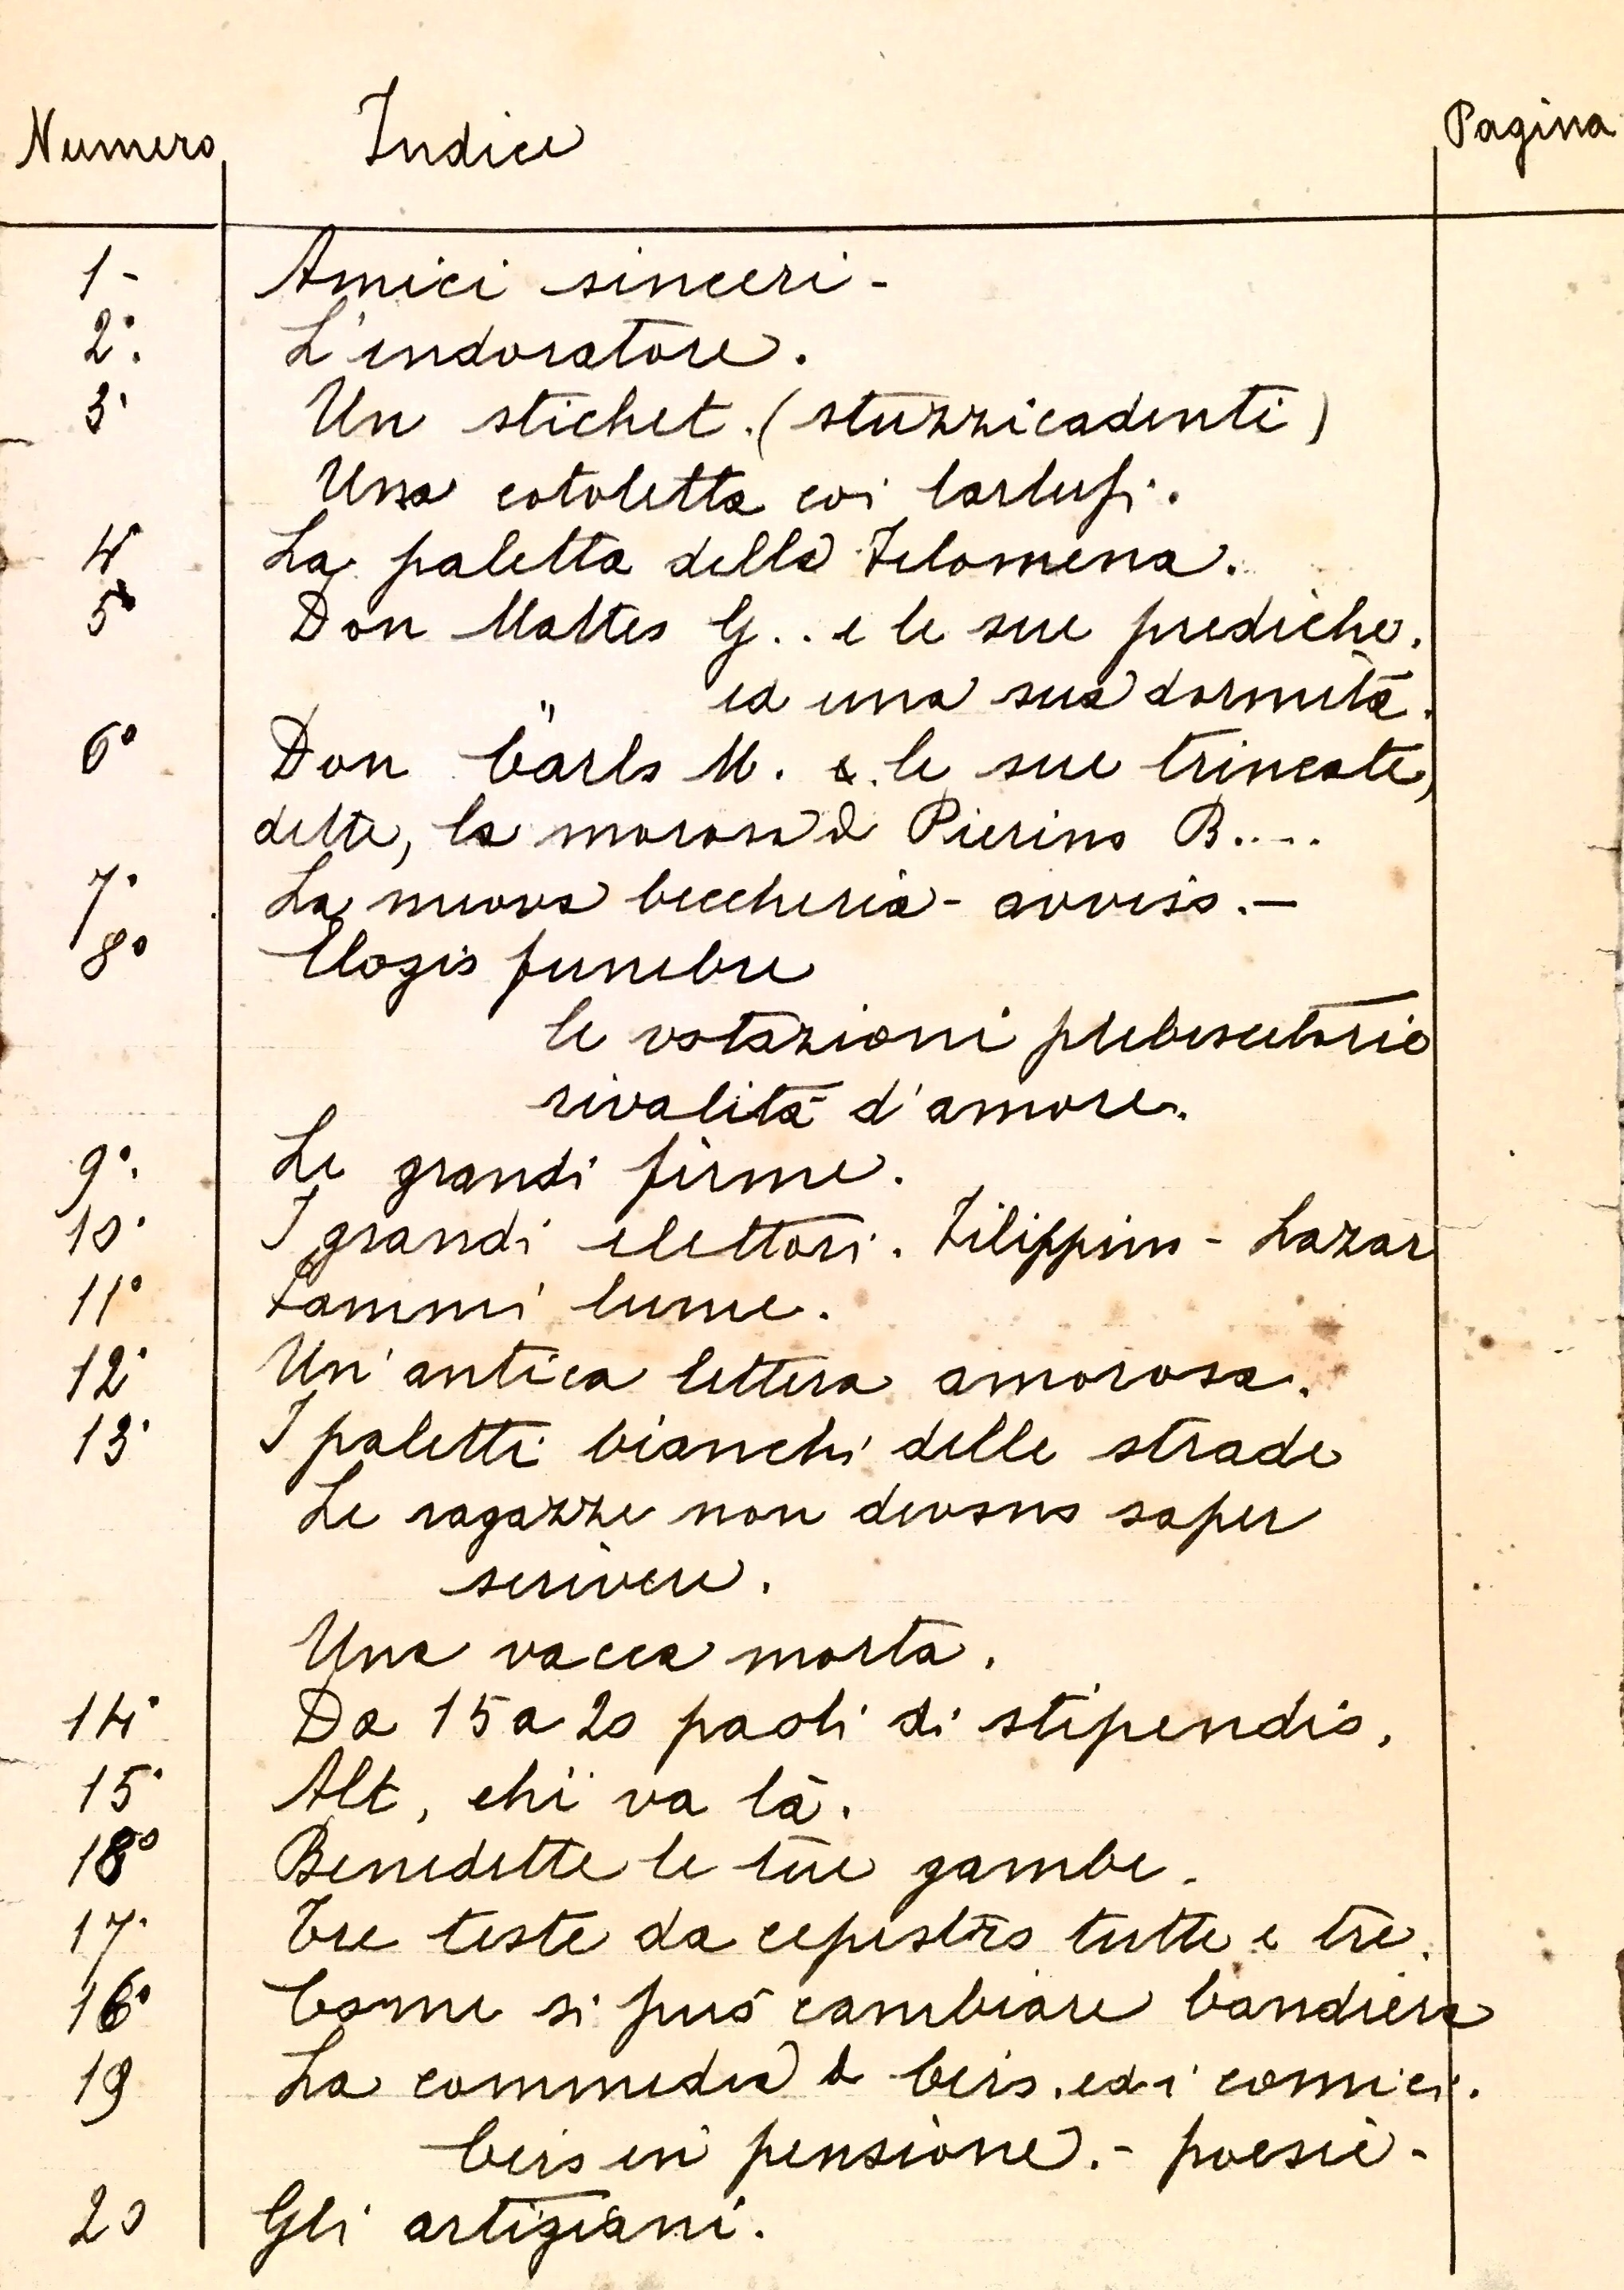
\includegraphics[width=0.98\textwidth]{indice}
    %\vspace{-0.3cm}t
\end{figure}
\newpage
\noindent Il dialetto scritto da Mingazzi è vistosamente approssimativo: spesso scrive in modi diversi una stessa parola e spesso dimentica accenti necessari per la comprensione. D'altronde è risaputo che il dialetto romagnolo è una lingua relativamente facile da parlare ma di difficile scrittura. Per questo motivo ho aggiunto un minimo di punteggiatura per una buona comprensione, senza però alterare le parole originali, in modo da osservare eventuali diversità tra il dialetto odierno e quello di un tempo. Voglio precisare che molte delle traduzioni in italiano delle frasi in romagnolo, sono state date direttamente da Mingazzi nel testo, tra parentesi. Mi sono limitato a riportare queste traduzioni, tali e quali, nelle note. Una modifica consistente riguarda le citazioni di scritti e di epigrafi che ho riportato al centro della pagina, in corsivo. Per quanto riguarda i dialoghi, ho scelto di munirli di adeguata punteggiatura e di andare a capo quando necessario. Non ho mantenuto lo stesso criterio con cui Mingazzi mandava a capo il testo, ma ho diminuito il numero di questi interventi per motivi di spazio e di leggibilità.	\\\\
\label{fonti}
\noindent A pagina \pageref{Personaggi} ho riportato i personaggi che sono riuscito a riconoscere utilizzando (per ordine di utilizzo):
\begin{itemize}\itemsep2pt
\item{\emph{Storia di Alfonsine}, \index[Personaggi]{Pasi Romano}Romano Pasi}
\item{\emph{alfonsinemonamour.racine.ra.it}, Luciano Lucci\index[Personaggi]{Lucci Luciano}}
\item{\emph{Le Alfonsine, il volto e l'anima}, Giovanni e Maria Francesca Zanzi\index[Personaggi]{Zanzi Giovanni}\index[Personaggi]{Zanzi Mariafrancesca}}
\item{\emph{Quaderni Alfonsinesi}, nella biblioteca Orioli di Alfonsine}
\item{Registri delle Delibere del 1914 e del 1929, nella biblioteca Orioli di Alfonsine}
\item{\emph{I fèt dla veriëla}, Edda Forlivesi\index[Personaggi]{Forlivesi Edda}}
\end{itemize}

A pagina \pageref{Luoghi} ho riportato l'indice di tutti i luoghi presenti nel libro. Per i personaggi e i luoghi più interessanti, ho riportato una descrizione nelle note. Chiedo nuovamente al lettore di prestare attenzione alle note, per meglio comprendere il testo.\\

\vspace{1cm}

Un appello ai lettori esperti: vi prego di contattarmi senza problemi, all'indirizzo email \textit{andraghetti.l@gmail.com} nel caso in cui voleste consigliare qualche correzione o qualche nome mancante.\\

\rightline{Vi ringrazio e vi auguro una buona lettura.}
